%% LLT: Turn off some annoying warnings...
\RequirePackage{silence}
\WarningFilter{titlesec}{Non standard sectioning command}
\WarningFilter{scrreprt}{Usage of package}
\WarningFilter{scrreprt}{Activating an ugly workaround}

% **************************************************
% Document Class Definition
% **************************************************
\documentclass[%
	paper=A4,					% paper size --> A4 is default in Germany
	twoside=false,				% onesite or twoside printing
	openany,					% doublepage cleaning ends up right side
	parskip=full,				% spacing value / method for paragraphs
	chapterprefix=true,			% prefix for chapter marks
	11pt,						% font size
	headings=normal,			% size of headings
	bibliography=totoc,			% include bib in toc
	listof=totoc,				% include listof entries in toc
	titlepage=on,				% own page for each title page
	captions=tableabove,		% display table captions above the float env
	draft=true,				% value for draft version
]{scrreprt}%

% **************************************************
% Debug LaTeX Information
% **************************************************
%\listfiles

% **************************************************
% Information and Commands for Reuse
% **************************************************
\newcommand{\thesisTitle}{Morphological Paradigm Completion\\with LSTM Neural Models}
\newcommand{\thesisName}{Conor Stuart Roe}
\newcommand{\thesisDate}{\today}
\newcommand{\thesisVersion}{Draft 0\\Advisor: Jane Chandlee}


% **************************************************
% Load and Configure Packages
% **************************************************
\usepackage{subfig}
\usepackage{booktabs}
\usepackage[utf8]{inputenc}		% defines file's character encoding
\usepackage[english]{babel} % babel system, adjust the language of the content
\usepackage[textsize=footnotesize]{todonotes}   % allows todo notes
\usepackage[					% clean thesis style
	figuresep=colon,%
	sansserif=false,%
	hangfigurecaption=false,%
	hangsection=true,%
	hangsubsection=true,%
	colorize=full,%
	colortheme=bluemagenta,%
 LLT: Use biber if using UTF8 encoding
	bibsys=bibtex,%
	bibsys=biber,%
	bibfile=sources,%
	bibstyle=authoryear,%
]{cleanthesis}

% Maroon and grey theme:
\cthesissetcolor{cmyk}{0, 1, .7, .3}{.7, 1, .7, .3}

\usepackage{amsthm}
 
\theoremstyle{definition}
\newtheorem{definition}{Definition}
\theoremstyle{theorem}
\newtheorem{theorem}{Theorem}[section]
 \usepackage{algorithm}
 \usepackage{algpseudocode}
 \usepackage{mathtools}
 \usepackage{amsmath}
\usepackage{graphicx}
\usepackage{hyperref}
\hypersetup{					% setup the hyperref-package options
%	pdftitle={\thesisTitle},	% 	- title (PDF meta)
%	pdfsubject={\thesisSubject},% 	- subject (PDF meta)
%	pdfauthor={\thesisName},	% 	- author (PDF meta)
%	plainpages=false,			% 	-
	colorlinks=true,
    linkcolor=blue,
    filecolor=magenta,      
    urlcolor=cyan,			% 	- colorize links?
%	pdfborder={0 0 0},			% 	-
%	breaklinks=true,			% 	- allow line break inside links
%	bookmarksnumbered=true,		%
%	bookmarksopen=true			%
}

\urlstyle{same}

% **************************************************
% Document CONTENT
% **************************************************
\begin{document}

% --------------------------
% rename document parts
% --------------------------
%\renewcaptionname{ngerman}{\figurename}{Abb.}
%\renewcaptionname{ngerman}{\tablename}{Tab.}
\renewcaptionname{english}{\figurename}{Fig.}
\renewcaptionname{english}{\tablename}{Tab.}
\setstretch{1.5}

% --------------------------
% Front matter
% --------------------------
\pagenumbering{roman}			% roman page numbing (invisible for empty page style)
\pagestyle{empty}				% no header or footers
% !TEX root = ../thesis-example.tex
%
% ------------------------------------  --> cover title page
\begin{titlepage}
	\pdfbookmark[0]{Cover}{Cover}
	\hfill
	\vfill
	{\LARGE\thesisTitle \par}
	\rule[5pt]{\textwidth}{.4pt} 
	{\Large\thesisName}
	\vfill
	A thesis submitted in partial fulfillment of the requirements for the \\
	degree of Bachelor of Arts in Linguistics and Computer Science
	\vfill
	\textit{\large\thesisDate} \\
	Version: \thesisVersion \\
	\texttt{\thesisLink}
\end{titlepage}


% ------------------------------------  --> main title page
% \begin{titlepage}
% 	\pdfbookmark[0]{Titlepage}{Titlepage}
% 	\tgherosfont
% 	\centering

% 	{\Large \thesisUniversity} \\[4mm]
% 	\includegraphics[width=6cm]{gfx/Clean-Thesis-Logo} \\[2mm]
% 	\textsf{\thesisUniversityDepartment} \\
% 	\textsf{\thesisUniversityInstitute} \\
% 	\textsf{\thesisUniversityGroup} \\

% 	\vfill
% 	{\large \thesisSubject} \\[5mm]
% 	{\LARGE \color{ctcolortitle}\textbf{\thesisTitle} \\[10mm]}
% 	{\Large \thesisName} \\

% 	\vfill
% 	\begin{minipage}[t]{.27\textwidth}
% 		\raggedleft
% 		\textit{1. Reviewer}
% 	\end{minipage}
% 	\hspace*{15pt}
% 	\begin{minipage}[t]{.65\textwidth}
% 		{\Large \thesisFirstReviewer} \\
% 	  	{\small \thesisFirstReviewerDepartment} \\[-1mm]
% 		{\small \thesisFirstReviewerUniversity}
% 	\end{minipage} \\[5mm]
% 	\begin{minipage}[t]{.27\textwidth}
% 		\raggedleft
% 		\textit{2. Reviewer}
% 	\end{minipage}
% 	\hspace*{15pt}
% 	\begin{minipage}[t]{.65\textwidth}
% 		{\Large \thesisSecondReviewer} \\
% 	  	{\small \thesisSecondReviewerDepartment} \\[-1mm]
% 		{\small \thesisSecondReviewerUniversity}
% 	\end{minipage} \\[10mm]
% 	\begin{minipage}[t]{.27\textwidth}
% 		\raggedleft
% 		\textit{Supervisors}
% 	\end{minipage}
% 	\hspace*{15pt}
% 	\begin{minipage}[t]{.65\textwidth}
% 		\thesisFirstSupervisor\ and \thesisSecondSupervisor
% 	\end{minipage} \\[10mm]

% 	\thesisDate \\

% \end{titlepage}


% % ------------------------------------  --> lower title back for single page layout
% \hfill
% \vfill
% {
% 	\small
% 	\textbf{\thesisName} \\
% 	\textit{\thesisTitle} \\
% 	\thesisSubject, \thesisDate \\
% 	Reviewers: \thesisFirstReviewer\ and \thesisSecondReviewer \\
% 	Supervisors: \thesisFirstSupervisor\ and \thesisSecondSupervisor \\[1.5em]
% 	\textbf{\thesisUniversity} \\
% 	\textit{\thesisUniversityGroup} \\
% 	\thesisUniversityInstitute \\
% 	\thesisUniversityDepartment \\
% 	\thesisUniversityStreetAddress \\
% 	\thesisUniversityPostalCode\ and \thesisUniversityCity
% }
		% INCLUDE: all titlepages
 \cleardoublepage

%\pagestyle{plain}				% display just page numbers
% % !TEX root = ../thesis-example.tex
%
\pdfbookmark[0]{Abstract}{Abstract}
\chapter*{Abstract}
\label{sec:abstract}
\vspace*{-10mm}

		% INCLUDE: the abstracts (english and german)
% \cleardoublepage

% % !TEX root = ../thesis-example.tex
%
\pdfbookmark[0]{Acknowledgement}{Acknowledgement}
\chapter*{Acknowledgements}
\label{sec:acknowledgement}
\vspace*{-10mm}

This thesis would not have been possible without the feedback of my student readers Tessa Pham and Anya Capps and my second faculty readers Amanda Payne and Steven Lindell, nor without the guidance of Sorelle Friedler, professor of the Haverford Computer Science department's thesis seminar, but most of all it has been enabled by the continued support and guidance of my advisor, Jane Chandlee. % INCLUDE: acknowledgement
% \cleardoublepage

\setcounter{tocdepth}{2}		% define depth of toc
\tableofcontents				% display table of contents
 \cleardoublepage

% --------------------------
% Body matter
% --------------------------
\pagenumbering{arabic}			% arabic page numbering
\setcounter{page}{1}			% set page counter
\pagestyle{maincontentstyle} 	% fancy header and footer

% \chapter{Introduction}
\label{introduction}

\section{Section Name}

\subsection{Subsection Name}




\chapter{Theoretical background}

\section{Natural language morphology and typology}

\subsection{What is natural language morphology?}

One way that human languages express grammatical or semantic meaning is by altering individual words; this process is called \textbf{morphology}. Linguistic morphology is split into two major categories: \textbf{inflectional} and \textbf{derivational}. Inflectional morphology comprises alterations to words that reflect \textit{grammatical} meaning, that is, it indicates which of a determined subset of grammatical categories is at work in a particular phrase. For example, the verb \textit{paint} is grammatically inflected in the sentence \textit{"He paints."} to indicate agreement with a third-person singular subject. Derivational morphology applies \textit{semantic} alterations, that is, it shifts the fundamental meaning of a word, often switching its part of speech. For example, the verb \textit{paint} can become the noun \textit{painter}, denoting a person characterized by performing the action of the verb \parencite{Hogan2010}. 

The concept of \textbf{part of speech} refers to high-level groupings of words within a language according to what inflectional morphology they may undergo. Common parts of speech include nouns, verbs, and adjectives, although the exact division of parts of speech is language-specific. Within a given language and part of speech, there is typically a well-defined, finite set of \textbf{forms} that a given word may take; that abstract set of forms is called a \textbf{paradigm}. In particular, there is typically a set of \textbf{morphological categories} associated with a given part of speech in a given language. Common examples of morphological categories include number (e.g., singular vs. plural), verb tense, and noun or pronoun case (English exhibits case only in pronouns: I, me, my). Inflection is then used to assign a value to some or all of the morphological categories for a given word \parencite{Hogan2010}. For example, Spanish adjectives such as \textit{pequeño} "small" inflect for gender and number:

\begin{center}
\begin{tabular}{|c||c|c|}
\hline
& singular & plural \\
\hline \hline
masculine & \textit{pequeño} & \textit{pequeños} \\
\hline 
feminine & \textit{pequeña} & \textit{pequeñas} \\
\hline
\end{tabular}
\end{center}

 The term "word" can be ambiguous when speaking of linguistic morphology. To be more specific, a \textbf{form} is a word with a specific spelling or pronunciation and corresponding to a specific set of grammatical values, e.g., a single cell in the above table. The set of forms across an entire inflectional paradigm are said to belong to the same \textbf{lexeme}. A lexeme can be identified by its \textbf{lemma} - a citation or dictionary form, a particular cell in the paradigm that is chosen to represent the entire lexeme. Spanish adjectives are usually cited in the masculine singular, so the above forms may be said to belong to the Spanish lexeme that has the lemma \textit{pequeño} \parencite{Hogan2010}.

In contrast, derivational morphology is applied in a less systematic manner, and constraints on its application are as often semantic or idiosyncratic as determined by part of speech or other formal categories. For example, the English verb \textit{like} may become the common derived term \textit{likeable}, but an analogous term \textit{hateable} is much less often seen. For this reason, derivational morphology is more difficult to systematically study; this paper is only concerned with inflectional morphology.

An important concept in morphology is that of \textbf{inflection classes} - subgroupings of parts of speech in a given language that exhibit similar patterns of inflection to one another. An example the division of Spanish verbs into \textit{-ar}, \textit{-er}, and \textit{-ir} classes:

\begin{center}
\begin{tabular}{|c|c|c|c|}
\hline
infinitive & 3rd person sg. imperfect indicative & gerund \\
\hline \hline
\textit{bailar} & \textit{bailaba} & \textit{bailando} \\
\hline 
\textit{comer} & \textit{comía} & \textit{comiendo} \\
\hline 
\textit{partir} & \textit{partía} & \textit{partiendo} \\
\hline 
\end{tabular}
\end{center}

Many types of grammatical categories commonly appear cross-linguistically, such as number, gender, animacy, case, politeness, tense, aspect, mood, and definiteness. The values that these categories may take often differ somewhat in meaning from language to language (for instance, English only has one inflected past tense while Spanish has two), but the parallels between them are typically enough that it's possible to make general characterizations of the degree of similarity of inflection systems between to languages. English and Spanish both inflect nouns for singular and plural number, and neither inflects nouns for case, but Spanish can inflect some human nouns for gender as well, and inflects adjectives for number and gender where English adjectives are not \parencite{Hogan2010}. A related notion is that of paradigm size. English nouns only ever take two forms - singular and plural - while Finnish nouns may take about 28 \parencite{Wiktionary}.

\subsection{Types of inflection}

There are many \textbf{inflection shapes} seen in natural languages. The most basic is \textbf{affixation}: the addition of sounds to the beginning, middle, or end of a word. Affixation can be broadly divided into prefixation (addition of an affix to the beginning of a word), suffixation (to the end), infixation (in the middle), circumfixation (at both ends). Other designations for affixation shapes include ablaut (alteration or replacement of a sound in the middle of a word) and templatic morphology. Templatic morphology is a complex process by which certain elements of a stem are distributed throughout a form, interwoven with elements indicating grammatical value. 

\textbf{Fusion} refers to the marking of multiple categories at once with a single indivisible morpheme, e.g., the Spanish verb \textit{hablé} "I spoke" marks tense and subject person and number with the suffix \textit{-é}, lacking separable morphemes to indicate the preterite tense and first person singular subject (cf. \textit{hablo} "I speak", \textit{habló} "he/she spoke"). 

\begin{center}
\begin{tabular}{|c||c|c|}
\hline
& 1st person singular & 3rd person singular \\
\hline \hline
present & \textit{hablo} & \textit{habla} \\
\hline 
preterite & \textit{hablé} & \textit{habló} \\
\hline
\end{tabular}
\end{center}

\textbf{Reduplication} is the repetition of all or part of a word. Reduplication may be full, as in Indonesian \textit{orang} "person" vs. \textit{orang-orang} "people", or partial, as in the formation of the contemplative aspect of the Tagalog word \textit{bili} "buy" by repeating the first syllable: \textit{bibili} (examples from Wiktionary). 

\textbf{Long-distance morphophonological processes} are those by which the surface form of an affix depends on the phonological properties of a segment at some distance from the affixation site. For instance, Finnish exhibits vowel harmony, a process by which the vowels present in affixes depend on the set of vowels in the stem. The Finnish inessive singular suffix \textit{-ssa/-ssä} looks different on the nouns \textit{puku} "suit" and \textit{kenkä} "shoe", with the final vowel of the suffix dependent on the set of vowels in the rest of the word. 

\begin{center}
\begin{tabular}{|c|c|}
\hline
nominative singular & inessive singular \\
\hline \hline
\textit{puku} & \textit{puvussa} \\
\hline 
\textit{kenkä} & \textit{kengässä} \\
\hline
\end{tabular} \\
\vspace{.3cm}
\parencite{Wiktionary}
\end{center}

Lastly, \textbf{irregularity} is a concept with familarity to anyone who's ever tried to learn a foreign language. Forms or entire lexemes are said to be irregular if they are aberrant from the normal patterns of morphology. For example, almost all English verbs only mark a third person singular subject differently from others, with a suffix \textit{-s}: \textit{I run} but \textit{she runs}. However, \textit{to be} marks the first person singular subject differently as well, and the third person singular subject marking bears no resemblance to the normal affixation process: \textit{I am}, \textit{you are}, \textit{she is}. It can be said that \textit{be} is a highly irregular verb.

\subsection{Linguistic typology}

\textbf{Linguistic typology} refers to the classification of languages into different categories depending on their structure. The major categories of morphological typology are \textbf{isolating}, \textbf{agglutinating}, and \textbf{fusional}. Languages are considered to be more isolating if they have little grammatical inflection, smaller inflection paradigms, and a smaller number of affixes per word on average \parencite{Hogan2010}. English is a fairly isolating language, likely a factor in the lack of computational morphology research \parencite{Cotterell2017}. Languages are considered to be more agglutinating if they exhibit more extensive inflection but do not typically exhibit fusion; agglutination is also associated with greater morphological regularity. Fusional languages are simply those that exhibit relatively more fusion. Like many typological distinctions, there is no strict assignment of languages into one or another of these categories; rather, they are ends of a spectrum that languages may be placed along \parencite{Hogan2010}.

Other typological labels may be applied depending on the set and shape of morphological inflection. Languages may be considered \textbf{highly inflecting} or \textbf{polysynthetic} if they have very large morphological paradigms. Languages may be typified by the presence of grammatical gender, vowel harmony, or other morphological characteristics. In general, this study is not concerned with defining specific labels for languages so much as computationally measuring the structural similarity of their morphological systems.

\subsection{Linguistic genealogy}

\begin{figure}[ht]
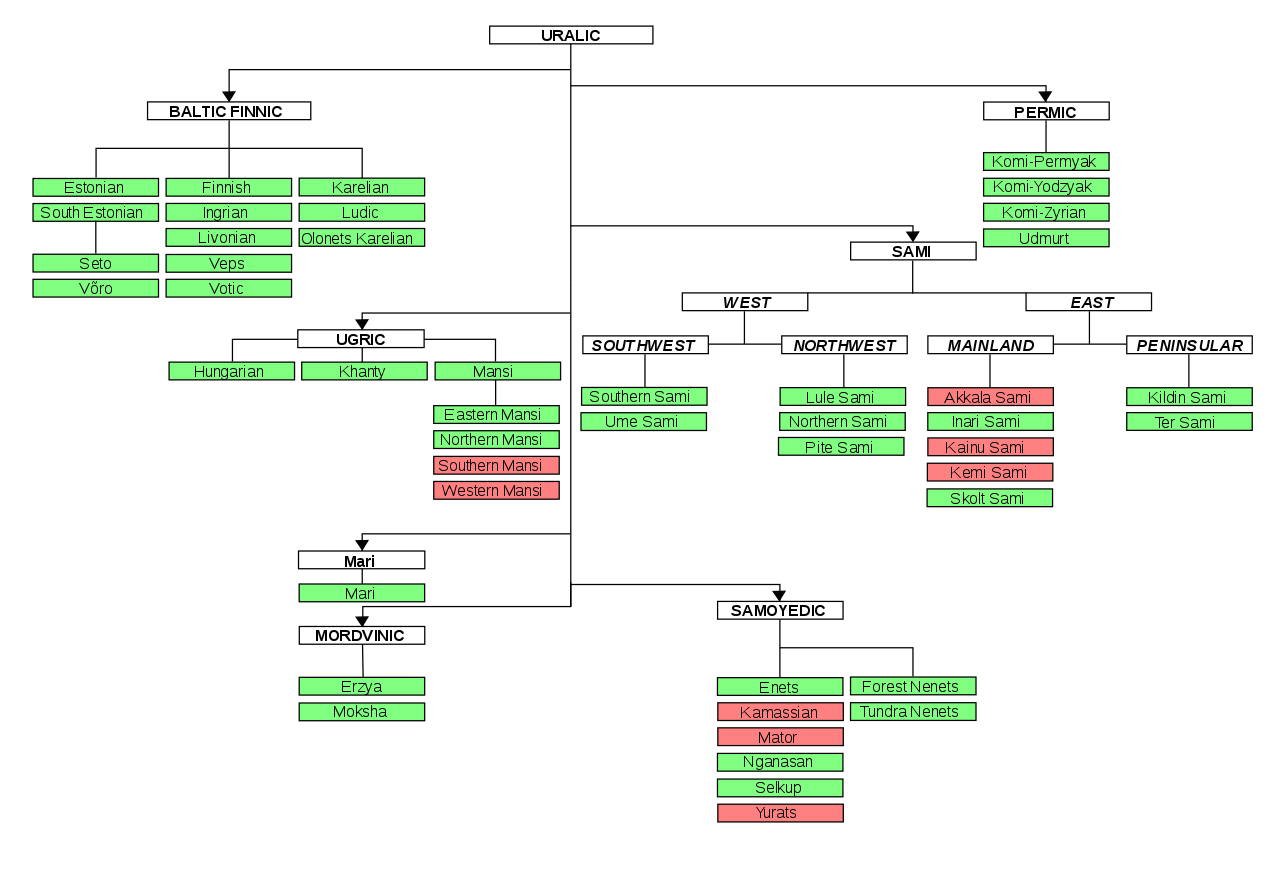
\includegraphics[width=13cm]{images/1280px-UralicTree.png}
\centering
\caption{The entire Uralic language family. \\ (commons.wikimedia.org/wiki/File:UralicTree.svg)}
\end{figure}

Languages change and diverge over time, and their development tends to follow genealogical patterns analogous to species descent and divergence. They are commonly grouped into \textbf{language families}, described with genealogical trees, and genealogical distance can be measured between them.

Language relationships are ascertained via historical comparison, and language families are simply the largest possible groupings that can be supported with certainty by available evidence. As such, they are not alike in historical timescale or internal diversity; more well-studied or attested families, and those with more historical written material, are likely to be larger because there is information available with which to make inferences about language descent in the distant past.

For this reason, a simple measure of genealogical separation cannot easily be come by. Relative location in a language family tree may not be informative, since the number of members and the density of branching differs between families. Another strategy is to measure \textbf{lexical similarity}: the proportion of words between two languages which are obviously similar due to shared origin.

However, lexical similarity is a measure of the similarity of vocabulary items and is not a good proxy for the grammatical similarity of languages. English has borrowed a very large amount of vocabulary from various historical varieties of French, yet their morphological systems remain fairly faithful to their respective origins in different branches of the Indo-European family. French in particular bears substantial morphological similarity to other Western Romance languages like Spanish and Portuguese. Even languages with no known genealogical relationship and extremely different grammatical systems may have non-zero lexical similarity: Turkish and Urdu have both borrowed heavily from Arabic, yet the grammatical systems of the three languages are quite distinct.

\section{LSTM and GRU neural modeling}
\label{sec:LSTM}

\begin{figure}[p]
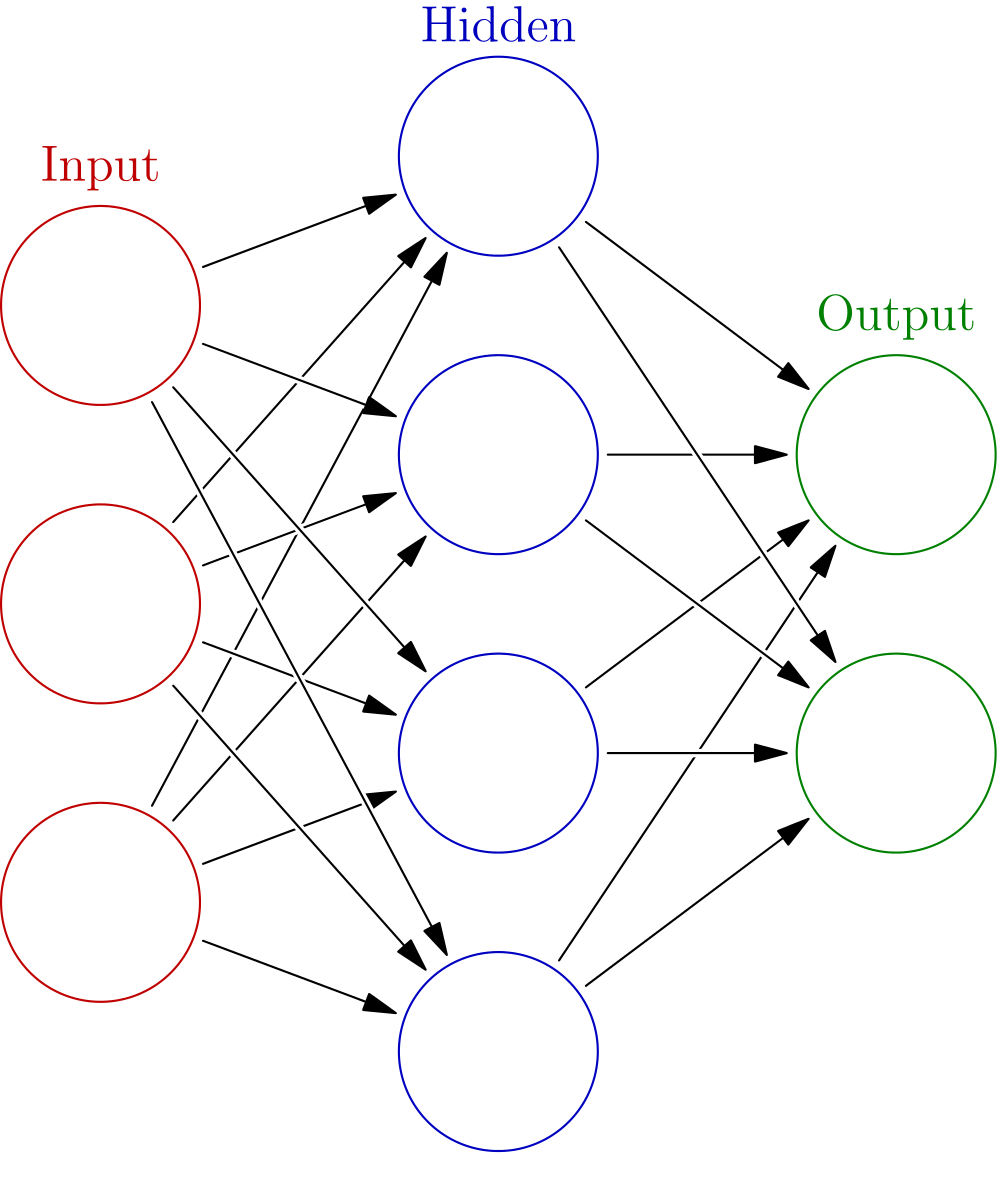
\includegraphics[width=6cm]{images/1000px-Colored_neural_network.png}
\centering
\caption{The structure of a feed-forward neural network with three inputs, four hidden cells, and two outputs. \\ (commons.wikimedia.org/wiki/File:Colored\_neural\_network.svg)}
\label{fig:NN}
\end{figure}

\begin{figure}[p]
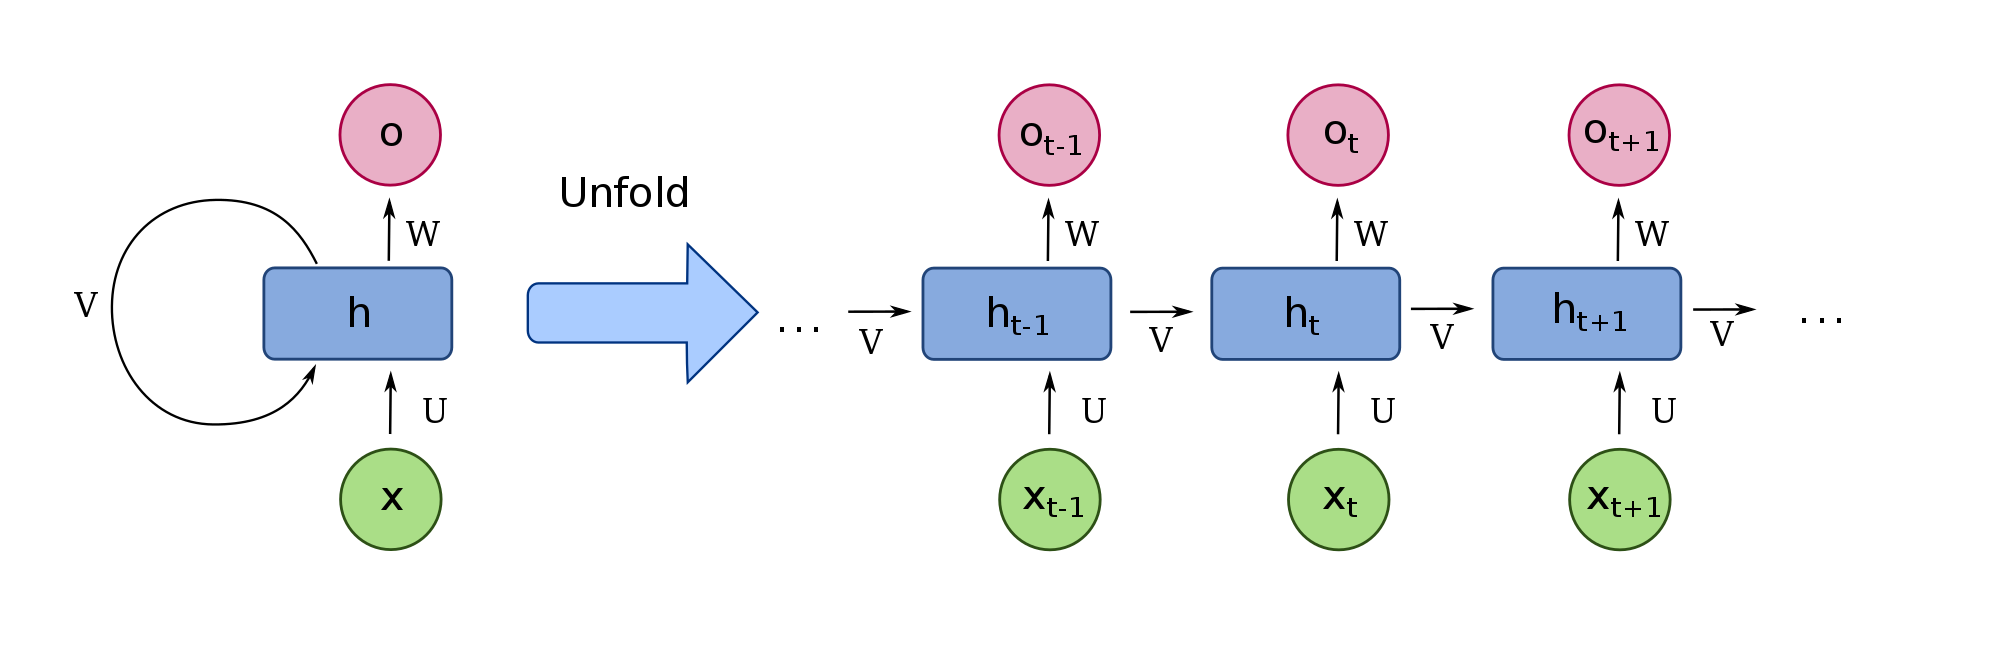
\includegraphics[width=12cm]{images/RNN.png}
\centering
\caption{The generalized structure of a recurrent neural network. \\ (commons.wikimedia.org/wiki/File:Recurrent\_neural\_network\_unfold.svg)}
\label{fig:RNN}
\end{figure}

\begin{figure}[p]
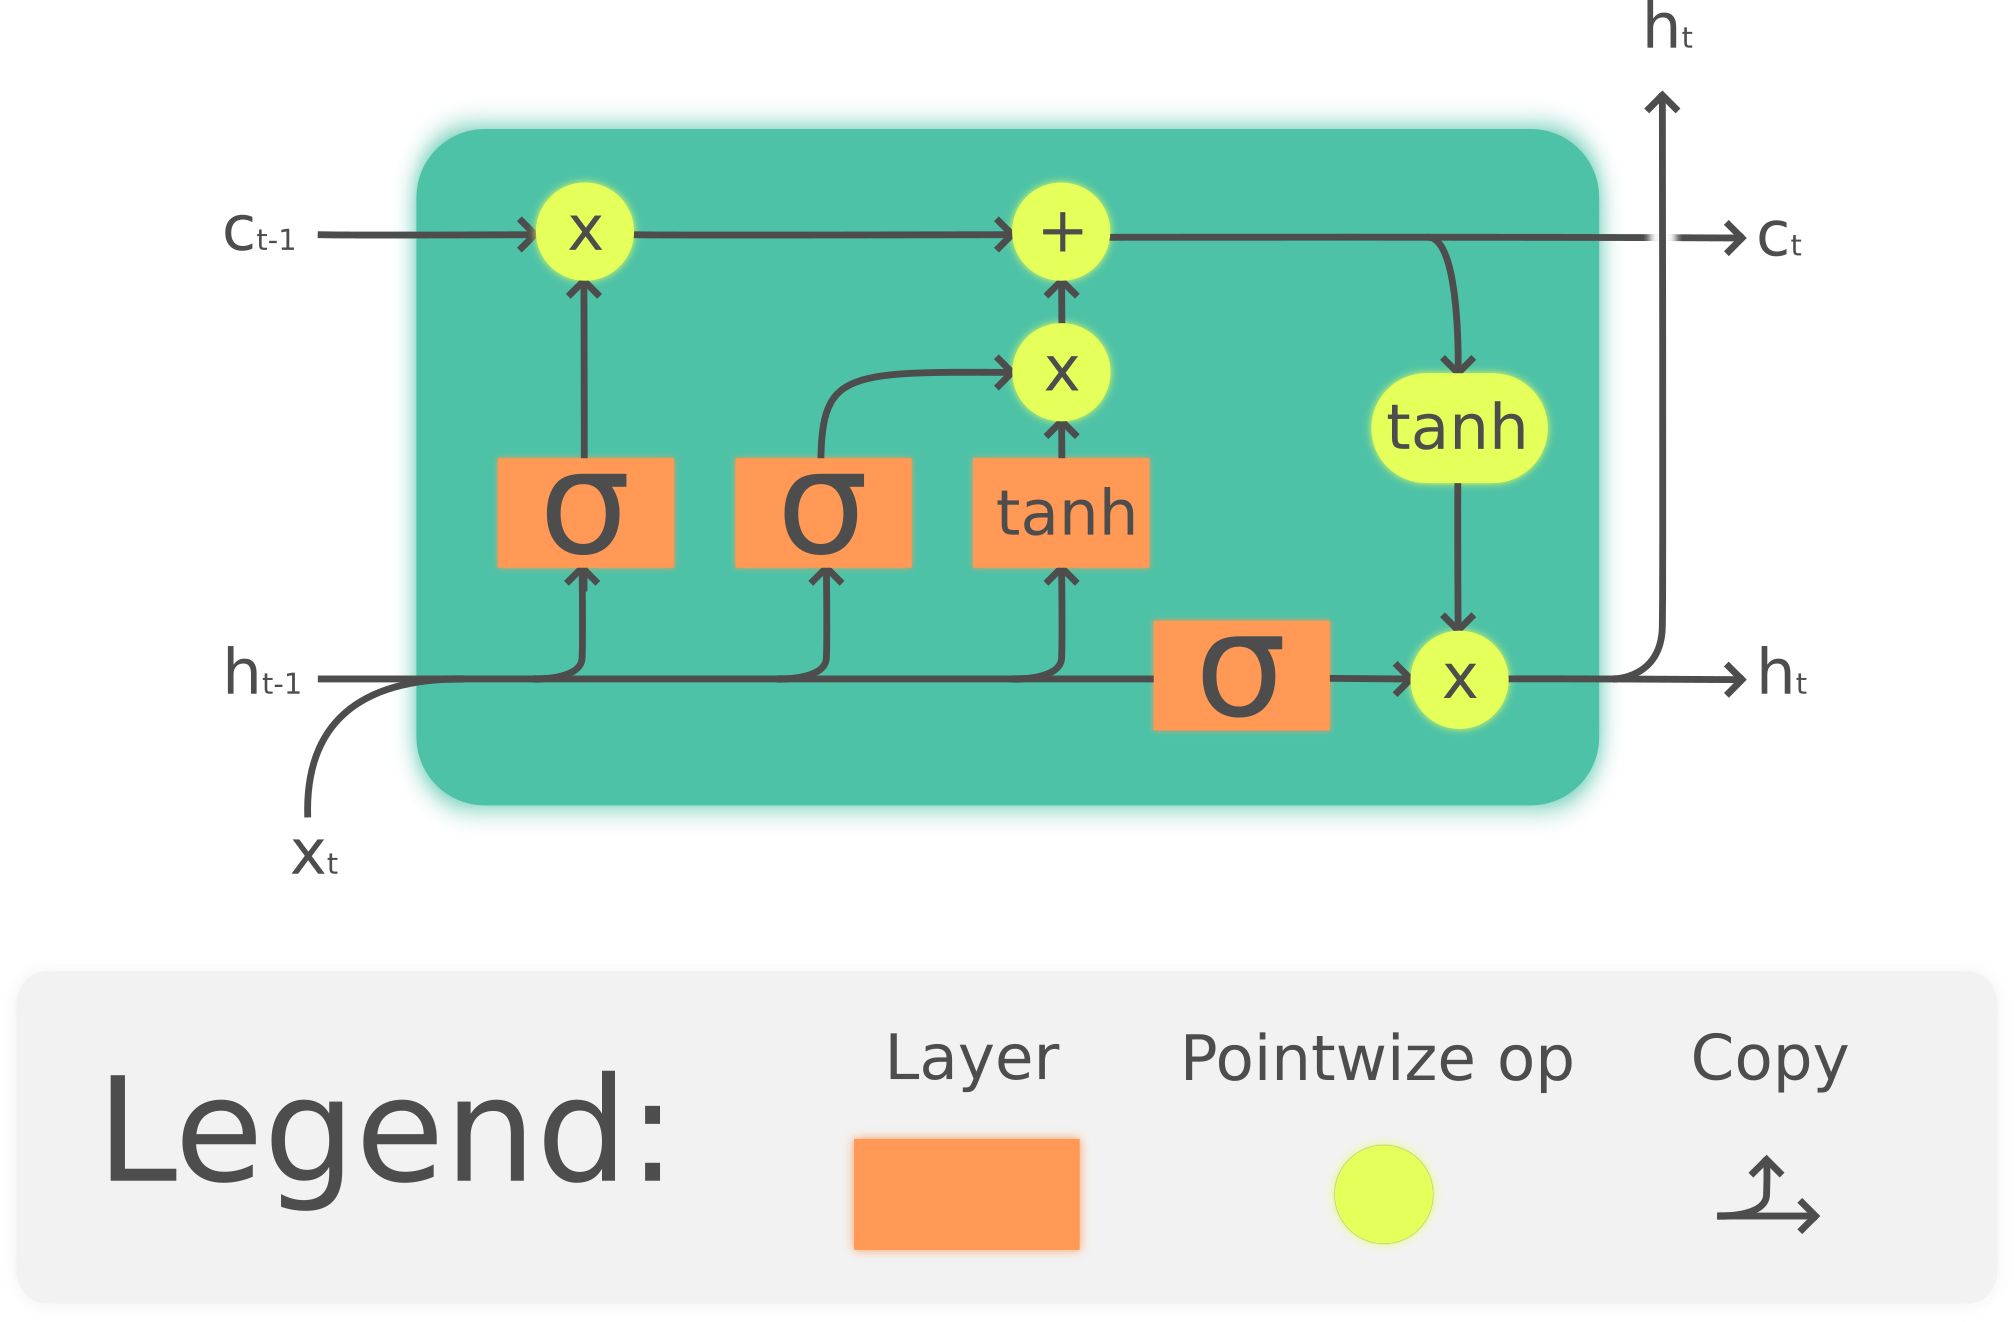
\includegraphics[width=12cm]{images/The_LSTM_cell.png}
\centering
\caption{The state cell of an LSTM model. \\ (commons.wikimedia.org/wiki/File:The\_LSTM\_cell.png)}
\label{fig:LSTM}
\end{figure}

\textbf{Neural networks} are a type of function approximation model inspired by the connection of neurons in animal brains. They have come to be implemented in a variety of forms, and underlie state of the art machine learning models in a variety of applications. The common feature of neural models is repeated matrix multiplication followed by the application of a non-linear "activation" function. Fig. \ref{fig:NN} illustrates a simple feed-forward network, in which a vector of three inputs is multiplied by some $3 \times 4$ matrix and activated to produce a vector of four intermediate values, which are again multiplied by some $4 \times 2$ matrix and activated to produce a vector of two outputs.

A \textbf{recurrent neural network (RNN)} is a type of neural network that operates over sequences of inputs, typically with unknown length. Fig. \ref{fig:RNN} illustrates the general structure: each input is represented by a vector, which is multiplied by a vector $U$ to modify state, and the modified state is then multiplied by a vector $W$ to produce an output vector and a matrix $V$ to produce the next state. 

\textbf{Long short-term memory (LSTM)} neural networks are a variant of RNNs which use a more complex sequence of computations to update state, and maintain a separate piece of state \textit{c} that controls rate of forgetting. LSTMs are intended to solve the forgetfulness of more basic RNN types, which tend to be unable to recall information from more than a few iterations prior \parencite{Hochreiter1997}. LSTM architecture is described in Fig. \ref{fig:LSTM}: the input $x_i$ and the previous state $h_{i-1}$ are linearly transformed, added, and activated, as in a simple RNN, before interacting via a series of operations with the previous cell $c_{i-1}$, producing the next state $h_i$ and cell $c_i$. \textbf{Gated recurrent units} (GRU) are slightly simplified models that do not include separate parameterization of the output gate (not pictured).

LSTMs have become the dominant model type in a variety of language tasks, including syntactic and morphological tasks. They significantly outperformed other types of models in SIGMORPHON 2016, since which time they have come to underlie nearly all morphology prediction models (\cite{Cotterell2016}, \cite{Cotterell2017a}).

\begin{figure}[ht]
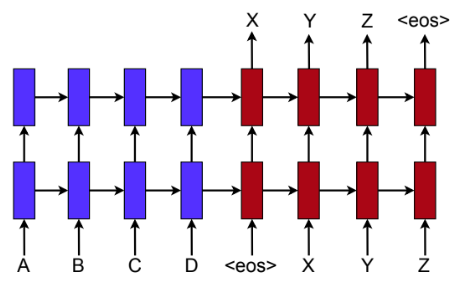
\includegraphics[width=10cm]{images/stacked.png}
\centering
\caption{A stacked RNN architecture, in which there are two layers of hidden state. In this architecture, hidden states in the second layer are exclusively derived from the aligned cell of the first layer. \parencite{Luong2015}}
\end{figure}

\begin{figure}[p]
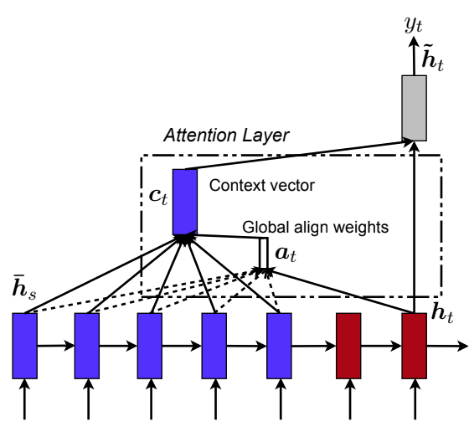
\includegraphics[width=10cm]{images/global.png}
\centering
\caption{An RNN architecture with global attention: all first-layer hidden states are used to construct an output. \parencite{Luong2015}}
\label{fig:global}
\end{figure}

\begin{figure}[p]
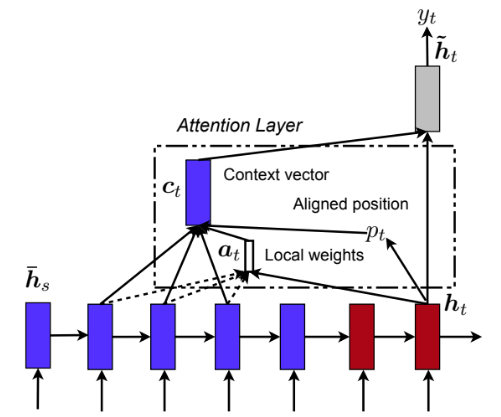
\includegraphics[width=10cm]{images/local.png}
\centering
\caption{An RNN architecture with local attention: only a subset of hidden states, not necessarily contiguous, are used to construct an output. \parencite{Luong2015}}
\label{fig:local}
\end{figure}

The main differences between the LSTM architectures used in state of the art applications now, as evidenced by the four architectures used as baselines in the SIGMORPHON 2019 transfer learning task, are in their \textbf{attention mechanism}, the means by which hidden states are combined to generate sequential output \parencite{Cotterell2019}. 

The main contrasting terminologies for attention are \textbf{hard} vs. \textbf{soft}, and \textbf{global} vs. \textbf{local}. In soft attention models, hidden states are all considered, weighted using an additional layer. In hard attention models, only a limited subset of hidden states are considered, the selection of hidden states may be chosen by the model at each stage or consist of a single sliding window of attention. Soft attention models are straightforward to apply backpropagation to, since each hidden state has a differentiable relationship to the output, while hard attention models that select which hidden states are used at a particular time step are not. A \textbf{monotonic} hard attention model is one in which the window of attention moves through the input at the same rate that the output is generated, which is applicable in scenarios when corresponding positions in input and output are expected to be strictly related. \textbf{Global} vs. \textbf{local} attention refers to whether all or only a narrow range of hidden states contribute to a hard attentional layer, as depicted in Figs. \ref{fig:global} and \ref{fig:local} \parencite{Luong2015}. 

\section{Transfer learning}

Transfer learning is a high-level term for any machine learning process for which either the domain or the distribution of some or all training data inputs is different from that of the inputs to which a model will ultimately be applied. Such techniques arise in response to the conundrum that many real-world machine learning problems face: a lack of data that looks like the system that one wishes to predict or understand, either due to insufficient available quantity, or altogether lack in the case of seeking to predict the outcome of future events of which no past equivalents exist. The machine learning problem for which a model is initially trained is called the \textbf{source task}; the problem which the model is being constructed to solve is called the \textbf{target task}. Typically, the source model is not the only component of the eventual target model - manual output transformations or additional machine learning is usually applied \parencite{Pan2010}.

\begin{figure}[t]
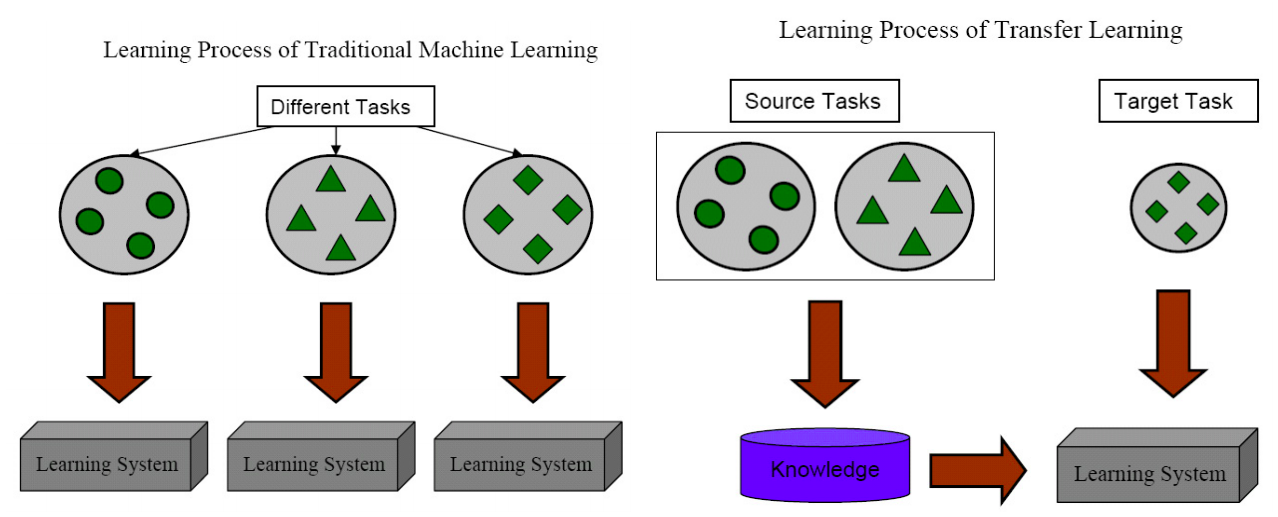
\includegraphics[width=12cm]{images/transfer_learning.png}
\centering
\caption{An abstract characterization of traditional ML vs. transfer learning}
\end{figure}

Some examples are provided by Pan and Yang 2010. One is the problem of seeking to classify web documents by topic. If a significant portion of the documents that will need to be classified bear on topics rarely covered in an existing corpus of web documents, this is an example where the training and test domains are roughly similar but their distribution is different; it is perhaps a less obvious transfer learning problem. Another example is that of attempting to gauge sentiment of reviews of cameras, when the only available data is a corpus of reviews of other types of products. In this case, knowledge of many domains, none of which is equal to the target domain, must be transferred to attempt to make predictions about the target domain.

There are three broad categories of transfer learning that Pan and Yang identify, which differ in their intrinsic difficulty. \textbf{Inductive transfer learning} describes a modeling scenario in which the domains of source and target are identical, but the target task is different, that is, the codomain of the model differs. In inductive transfer learning, output from the source model is used to inform a model of the target task. \textbf{Transductive transfer learning} describes the scenario that the task is the same but the source and target domains are in some way different, either differing in feature space, or having the same feature space but differing in distribution over that space. The two examples above are both instances of transductive transfer learning; the web document categorization problem is an example of differing distribution while the review sentiment analysis problem is an example of differing feature space. \textbf{Unsupervised transfer learning} describes the scenario that source and target differ in both domain and codomain. 

An example of unsupervised transfer learning is the morphology transfer learning problem that this thesis undertakes: labeled training inputs and outputs from the source (one language) are used to inform a model of the target task (a different language), and the feature spaces of both domain (lexemes and morphological categories) and codomain (inflected forms) differ between the two. After all, no two languages share the same set of words, and only in the case of very closely related languages or extreme coincidence will all grammatical paradigms inflect for the same set of morphological categories (one language is likely to have a grammatical gender, a verb tense, or some other category that the other language lacks).

There is precedent for transfer learning on LSTMs for language technology tasks, typically with the explicit goal of dealing with low data volume in the target task due to sparse language resources. The baseline for SIGMORPHON 2019 was based on the LSTM transfer learning architecture introduced in Zoph et al. 2016 \parencite{McCarthy2019}, which was applied there to a transductive machine translation task. Their approach is relatively straightforward - they use an LSTM encoder-decoder model to train a machine translation system from French to English on a high data volume, then use that model as the initialization of an architecturally identical Uzbek-English model, holding the decoder fixed and simply allowing the encoder to learn encodings for Uzbek with quite a small dataset. Their results showed considerable improvements over similarly low-data machine translation techniques \parencite{Zoph2016}, suggesting that transfer learning may be a promising strategy for computational linguistics tasks.

\section{Ensembling}

\textbf{Ensembling} is another core ML concept that arises in explaining the differences in structure and performance of computational morphology models. It is a generic term for combining the outputs of multiple models which operate over the same domain and codomain. That is, ensembled models receive the same input, and produce outputs of the same form; their outputs are typically combined by vote in classification tasks or weighted or unweighted averaging in regression tasks. Ensembling among neural and non-neural models has been used to improve outcomes in a variety of tasks \parencite{Krogh1995}.

\chapter{Machine learning of morphology: existing work}

\section{Sub-problems and related problems}

Within the realm of machine understanding of morphology, there are many sub-problems and related problems. The most basic areas of research involve predicting the inflection morphology of words in isolation - transforming a word into a specific morphological form, or the inverse, tagging a form with its morphological categories. 

In this section, I used the machine learning terms \textbf{supervised} and \textbf{unsupervised}. Supervised learning is that conducted with labeled input-output sets, in which a model attempts to produce outputs similar to those it's seen. Unsupervised learning is that which attempts to find patterns in data sets with no output, such as finding clusters in a scatter plot of points. Note that this definition of \textbf{unsupervised} differs from the sense specific to transfer learning. The transfer learning task in SIGMORPHON 2019 is an example of an \textit{unsupervised} transfer learning problem in that the source domain and codomain are both different from target domain and codomain, yet it is \textit{supervised} in a general ML sense in that the triples included in the training data include output values which the model attempts to mimic.

\subsection{Core supervised learning problems}

Some of the earliest work in computational morphology involves making specific morphological transformations. That is, given a particular form of a lexeme (often, but not necessarily, a citation form), predicting another form. An example would be learning to transform English verbs from present to past tense, e.g., \textit{show} $\rightarrow$ \textit{showed}, \textit{see} $\rightarrow$ \textit{saw}, etc. \parencite{Dreyer2008}.

The natural extension of this is aiming to be able to predict any inflected form given one specific form of a lexeme and an arbitrary set of morphological categories. For instance, given a lexeme \textit{see} and the categories \texttt{3rd person singular, simple present}, generating the correct form \textit{sees}. Generally speaking, a citation form has been used as input (\cite{Durrett2013}, \cite{Faruqui2015}, \cite{Cotterell2017a}). The related "reinflection" problem involves being given any inflected form as input, and transforming it into any other \parencite{Cotterell2016}.

A further extension of the morphology generation problem is the generation of complete inflection tables. The exact nature of this problem depends on the type of training and test data used. If a model is only trained on a sparse, random sampling of forms for each lexeme, then a task may consist of filling out the rest of an inflection table for those lexemes. For instance, a model may be given the forms \textit{sees} and \textit{seeing} among its training data, and be required to fill out the remaining forms of that paradigm, including \textit{see} and \textit{saw}. If a model is instead trained using entire inflection tables, e.g., all forms of the verb \textit{see}, then test data must consist of new lexemes (\cite{Hulden2014}, \cite{Ahlberg2015}, \cite{Cotterell2017a}).

\subsection{Inflection types}

Overall, a diverse set of inflection shapes have been worked with in the most recent efforts of this subfield. Since 2016, the Special Interest Group on Computational Morphology and Phonology (SIGMORPHON), a research collective focused on computational morphology and related problems, has fielded "shared tasks" in which several research teams globally are given training data and a task definition, and attempt to create models which are subsequently compared. The SIGMORPHON shared task 2018 included training data from 103 typologically diverse languages, and paradigms using suffixing, prefixing, infixing, reduplication, and non-concatenative morphology. 

\subsection{Related problems}

Within only the last two or so years, there has been work on predicting morphology in context. In the 2018 and 2019 SIGMORPHON shared tasks, to which several teams of researchers submitted solutions, a sub-task was dedicated to cloze challenges, a type of test in which one word in a sentence, given in citation form, was to be inflected based on context (\cite{Cotterell2018b}, \cite{McCarthy2019}). This work is essentially a synthesis of morphology generation and morphosyntactic modeling.

Since 2017, there has been some work done on learning curves for computational morphology. The datasets published for SIGMORPHON 2017 and 2018 include partitions into low ($\sim$100 forms), medium ($\sim$1000 forms), and high ($\sim$10,000 forms) data training sets for the express purpose of assessing the learning curve of different models. Evidence suggests that learning curve varies by model type. LSTMs are generally the most accurate morphology models with high-data training sets and are considered state of the art. However, LSTMs and related neural model types often fare worse than more baseline string transduction models with small training sets, likely due to the very gradual gradient descent process used to fine-tune them (\cite{Cotterell2017a}, \cite{Cotterell2018b}). Improving performance with small training sets is of interest, as much of the applicability of computational morphology models is to languages which don't already have high-quality technical tools or datasets. 

The most recent new challenge that SIGMORPHON has tried to address is that of transfer learning of morphology, in the shared task earlier this year. Given a state of the art model trained on a language with a high volume of training data, teams were asked to alter it into a model that would perform well on a new language, given a smaller amount of training data for that language. 80\% of the pairs of languages were closely related, while 20\% were distantly or not at all related. Gains of transfer learning models between closely related languages were said to have generally performed better than transfer learning models between more distant languages \parencite{McCarthy2019}, although that conclusion is be examined more closely in this study.

\section{Non-neural approaches}

\subsection{Vector embedding}

A technique that has found success in a variety of computational linguistics tasks is that of representing words in relatively low-dimensional vector spaces. That is, words are represented as a vector, a series of numbers of fixed length; the length of the vector is typically much smaller than the number of total known words. This has the intention of capturing semantic and syntactic content in a principled way - similarities between the numbers representing two words are expected to signify actual similarity in their meaning, and regular linear transformations between vectors should roughly correspond to specific semantic or grammatical changes. These vector representations can be generated via various unsupervised learning methods (\cite{Bilmes2003}, \cite{Alexandrescu2006}).

\begin{figure}[ht]
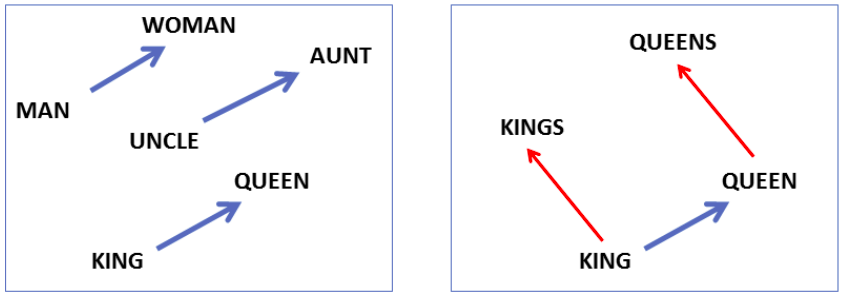
\includegraphics[width=12cm]{images/semantic_transform.png}
\centering
\caption{Regular spatial transformations encode semantic or grammatical content \parencite{Mikolov2013}}
\label{fig:vectors}
\end{figure}

Regularities in the relative location of semantically related words have been exploited for semantic analysis tasks \parencite{Alexandrescu2006}. Similarly, morphological changes may appear as spatial transformations in vector space, and work has been done on discovering morphological relationships between in-vocabulary words based on their relative spatial locations (\cite{Mikolov2013}, \cite{Soricut2015}, \cite{DosSantos2014}). Fig. \ref{fig:vectors}  illustrates this idea in a slightly simplified way: once a vector embedding model has been trained on English, it can be discovered that semantic transformations (male to female) and grammatical transformations (singular to plural) roughly correspond to regular spatial translations in vector space.

Vector embedding has the limitation that it cannot extend to words for which a vector representation has not been trained, and so it cannot directly provide understanding of the many OOV forms encountered in test data of highly inflected languages (\cite{Soricut2015}, \cite{Cotterell2019}). However, it can be a means to discover relationships between words in an unsupervised manner, which may support labeling tasks in support of computational morphology and other tasks.

\subsection{String transduction}

Earlier work specifically focused on the problem of morphology prediction made use of iteratively improving methods of string transduction - in essence, pattern matching on the written representations of words (\cite{Durrett2013}, \cite{Hulden2014}, \cite{Nicolai2015}, \cite{Ahlberg2015}). Typical steps of string transduction methods include character alignment (depicted in Fig. \ref{fig:chalign}), identification of characters that are inserted or deleted based on grammatical form, and generalization of lexemes which are inflected by the same sets of insertions or deletions (depicted in Fig. \ref{fig:transduction}). 

\begin{figure}[ht]
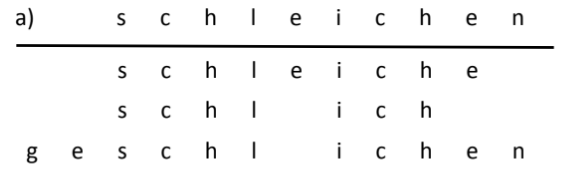
\includegraphics[width=12cm]{images/Nicolai2015_schleichen.png}
\centering
\caption{Character alignment for various forms of the German verb \textit{schleichen} \parencite{Nicolai2015}.}
\label{fig:chalign}
\end{figure}

\begin{figure}[ht]
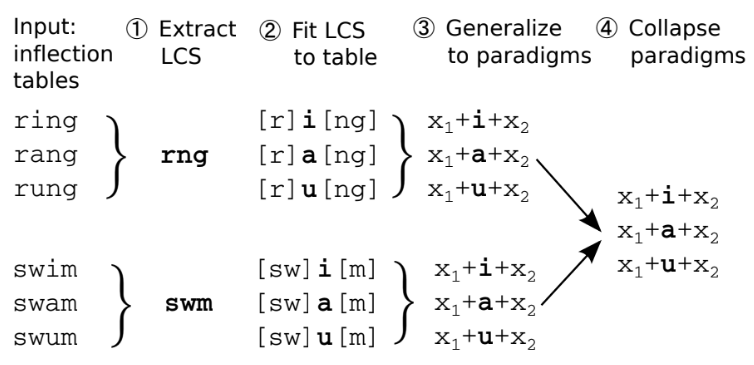
\includegraphics[width=12cm]{images/Hulden2014_diagram.png}
\centering
\caption{Conceptual depiction of a typical example of a string transduction method of morphology learning \parencite{Hulden2014}.}
\label{fig:transduction}
\end{figure}

A crucial limitation of string transduction methods are their general assumption that most lexemes have exactly the same set of characterwise transformations as a large group of other lexemes, and that a manageably small number of such inflection classes exist. There are paradigms with such a limited set of inflection classes, such as Spanish \textit{-ar}, \textit{-er}, and \textit{-ir} verbs. However, when multiple morpholonological processes are at play, individual lexemes may be nearly unique in their exact set of transformations.

For example, Finnish noun declension has processes of vowel harmony, consonant gradation, and vowel alternation and lengthening operating to produce final inflected forms \parencite{Ranta2008}. As an illustration, consider the Finnish nouns \textit{puku} "suit" and \textit{kenkä} "shoe", which have the inessive singular forms \textit{puvussa} "in the suit" and \textit{kengässä} "in the shoe", respectively. In both forms, the letter \textit{k} is transformed via consonant gradation, but the letter it becomes depends on the surrounding letters. The final vowel of the forms may be \textit{a} or \textit{ä}, depending on vowel harmony. In other inflected forms, the final vowel of the words may be doubled \parencite{Wiktionary}. A model that naively seeks to match these words with other words using the same set of character transformations across the paradigm may need to assign nearly every word to its own category, failing to generalize the patterns at work.

The poorer performance of string transduction relative to neural models has led to a move of the field away from string transduction since about 2016 \parencite{Cotterell2018b}.

\section{LSTM and other neural approaches}

Since 2016, almost all work on paradigm completion has made use of long short-term memory (LSTM) or related gated recurrent network (GRU) models (\cite{Faruqui2015}, \cite{Cotterell2016}, \cite{Cotterell2017a}, \cite{Cotterell2018b}, \cite{McCarthy2019}). An LSTM network is a variation on a recurrent neural network (RNN), a variant of neural network \parencite{Hochreiter1997}.

The SIGMORPHON 2019 transfer learning task used a diverse set of architectures as baselines, including a soft attention, a non-monotonic hard attention, and two monotonic hard attention models, reflecting a diversity of strategies employed by the best current models. Soft attention has dominated prior morphology learning work, but Wu and Cotterell (2019) demonstrate that hard monotonic models may be more appropriate for morphology tasks, where string transductions are mostly monotonic - that is, (except for in instances of reduplication or metathesis) characters in an input word correspond to characters in the same order in the output (\cite{McCarthy2019}, \cite{Wu2019}).

\section{Ensembling approaches}

\begin{figure}[ht]
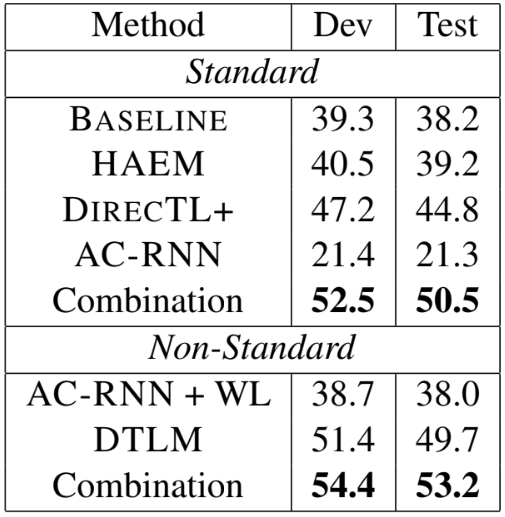
\includegraphics[width=7cm]{images/Najafi_accuracy.png}
\centering
\caption{The low-resource accuracy scores of the various University of Alberta models submitted to SIGMORPHON 2018 \parencite{Najafi2018}.}
\label{fig:Najafi}
\end{figure}

Ensembling was used in SIGMORPHON 2018 by various groups between neural and non-neural methods, specifically to ameliorate the poor performance of neural models in low-data settings \parencite{Cotterell2018b}. For example, the University of Alberta submission \texttt{UA-05} uses weighted voting to combine the 2019 baseline, a hard-attention LSTM model, a soft-attention LSTM model, and a string transduction model, favoring the output of generally more accurate models unless other models can agree on a different output. The \texttt{UA-08} system submitted by the same team combines the output of a string transduction and a soft-attention LSTM in a totally different way, by linear combination of their self-determined confidence scores \parencite{Najafi2018}.

Fig. \ref{fig:Najafi} shows the accuracy scores of the UA models averaged over all 103 languages of SIGMORPHON 2018 in the low-resource setting. \textsc{DirecTL+} and \textsc{DTLM} are string transduction models, \textsc{Baseline}, HAEM, AC-RNN, and AC-RNN + WL are LSTM models, and the two combinations are \texttt{UA-05} and \texttt{UA-08}, respectively; notice that the string transduction models score higher accuracy than neural models, but both ensembling methods have the highest accuracy of all.
\chapter{Data}

\section{Grammatical inflection data}

\begin{figure}[t]
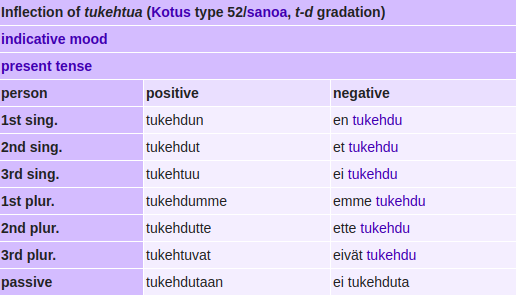
\includegraphics[width=12cm]{images/tukehtua.png}
\centering
\caption{The English Wiktionary partial inflection table for the Finnish word \textit{tukehtua}.}
\end{figure}

\begin{figure}[t]
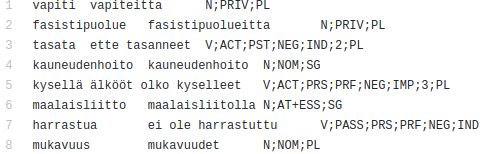
\includegraphics[width=12cm]{images/sigmorphon2018_fn.png}
\centering
\caption{A sample of the SIGMORPHON 2018 data for Finnish, scraped from Wiktionary and provided on GitHub (https://github.com/sigmorphon/conll2018/blob/master/task1/all/finnish-train-high).}
\end{figure}

I will be using the data set published for the SIGMORPHON first shared task 2018, which is publicly available on GitHub. It consists of triples - lemma, grammatical categories, and appropriately inflected form - for 103 languages, partitioned into training, development, and test sets. An example of some Finnish triples is shown in Figure 3.2. The training sets are further partitioned into low, medium, and high-resource sets; the low-resource training sets contain about 100 forms, medium about 1,000 forms, and high about 10,000 forms, with the sets being nested so that the smaller training sets are subsets of the larger ones. These data levels are used to simulate different resource settings, e.g., low-resource training sets represent data available for a poorly-resources language; the data levels can also be used to assess model learning curve \parencite{Cotterell2018b}.

\subsection{Language diversity}

The languages represented in the data cover a wide range of families and typological categories. Although over half of the languages are from the Indo-European family, a grouping that includes most languages of Europe, Greater Iran, and the northern part of the Indian subcontinent, one or more languages each of the Athabaskan, Kartvelian, Quechua, Semitic, Sino-Tibetan, Turkic, and Uralic families, as well as two isolates (Haida and Basque), are represented. Diverse inflection strategies are also represented, including suffixing, prefixing, infixing, ablaut, and introflexion, and long-distance processes like vowel harmony and consonant harmony \parencite{Cotterell2018b}.

\subsection{Sourcing and sampling}

The English Wiktionary, a collaborative online dictionary, has become something of a standard source of supervised morphological data. It provides full or partial inflection tables alongside lexeme definitions; the structure of tables is consistent for a given language and part of speech. An example table is given in figure 3.1. For some highly inflected languages (e.g., Navajo), Wiktionary only provides a fixed subset of forms. For some relationships between words that could be considered grammatical, it may simply offer them as separate lexical entries; for example, Russian perfect and imperfect forms are given as separate entries, as are Navajo verb forms that vary by aspect or thematic classifier \parencite{Wiktionary}.  

For most of the languages in the SIGMORPHON 2018 data, forms were gathered via scraping from Wiktionary. Multiple parts of speech are represented for most languages, but only parts of speech with a significant number of entries relative to all entries in a given language. Inflected forms were sampled for inclusion according to their estimated distribution in the text of Wikipedia for each respective language. For languages with sufficient data, 12,000 forms were sampled, and from these 1,000 were randomly selected for the development set and 1,000 for the testing set; the remaining 10,000 became the high-resource training set, of which 1,000 were randomly chosen as the medium-resource set and 100 of those as the low-resource set. For languages with less available data, sets might be smaller and the high-resource training set might be omitted; 17 languages lack high-resource sets \parencite{Cotterell2018b}.

\subsection{Representation of morphology}

The SIGMORPHON data set uses the UniMorph format to indicate grammatical categories  \parencite{Cotterell2018b}. The UniMorph project, initially published in 2015, is a format for encoding morphological categories uniformly cross-linguistically (\cite{SylakGlassman2015}, \cite{SylakGlassman2015a}, \cite{SylakGlassman2016}).

\section{Language typology data}

I will need numerical or categorical information about the morphological typology of the languages I consider in order to assess how typological similarities impact transfer learning. 

I may be able to gather some useful typological information the World Atlas of Language Structures (WALS), a linguistic typology database, and I also plan on generating my own typological data by computationally analyzing the SIGMORPHON 2018 data. WALS provides much of the same information that 

\subsection{Features}

The typological features I'm interested in considering include inflection shape (prefixing, suffixing, infixing, introflexion), set of inflected categories and overall paradigm size by part of speech, degree of fusion, and presence of long-distance phonological processes. 

Inflection shape may be important in determining, for instance, how soft attention models choose to focus on various parts of a word, so that a model trained on a language with a particular profile of inflection shapes may be more likely to attend to the correct parts of words when readapted to model a language with similar inflection shapes. 

Languages with similar sets of inflectional categories, e.g., languages which both mark adjectives for the gender and number of their head noun, or verbs with similar sets of tenses, may similarly benefit from transfer learning between them due to some form of model similarity. 

Fusion refers to the marking of multiple categories at once with a single indivisible morpheme, e.g., the Spanish verb \textit{hablé} "I spoke" marks tense and subject person and number with the suffix \textit{-é}, lacking separable morphemes to indicate the preterite tense and first person singular subject (cf. \textit{hablo} "I speak", \textit{habló} "he/she spoke"). Transfer learning may be beneficial between languages that both exhibit or lack fusion, or more specifically between languages that exhibit fusion between the same categories; since fusion operates over combinations of two or more categories, though, the space of possible fusion behaviors is quite large and it may be difficult to find unrelated languages with similar fusion behavior. 

Long-distance phonological processes are those by which the surface form of an affix depends on the phonological properties of a segment at some distance from the affixation site; consider my earlier example of vowel harmony in Finnish: the nouns \textit{puku} "suit" and \textit{kenkä} "shoe" have the inessive singular forms \textit{puvussa} "in the suit" and \textit{kengässä} "in the shoe", respectively, with final vowel of the suffix dependent on the set of vowels in the rest of the word. Given that long-distance processes present considerable difficulty for non-neural morphology models, neural models may have to be intensively trained to attend to such processes, presenting an opportunity for transfer learning to leverage existing knowledge.

I'd also like to take into account a more fine-grained measure of language relatedness, so that incidental typological similarities can be successfully statistically blocked against similarities arising from common origin. Two possible strategies are using detailed language genealogical trees and counting degrees of separation between languages, or finding some way to assess lexical similarity, the proportion of words between two languages which have both similar forms and meanings due to shared origin. Lexical similarity may be a more relevant measure - if word stems are similar between two languages, it is likely that grammatical affixes are as well. However, lexical similarity may also be due to shared areal loanwords, such as the profusion of Arabic loanwords into Turkish, Persian, and Urdu. Areal effects can also cause grammatical similarity to spontaneously arise between geographically collocated languages \parencite{Ponti2018}, though grammatical similarities due to shared ancestry are probably stronger. Ultimately, lexical similarity and genealogical closeness measure different types of linguistic relationships, and both should be taken into account if good data is obtainable.

Consistent and quite fine-grained information about language genealogy can be found on Ethnologue, a database of basic typological and socioliguistic information about all recognized languages \parencite{Ethnologue}. Finding good data about lexical similarity looks to be significantly more challenging - certainly, no database exists of pairwise lexical similarity between all languages, and automatically calculating lexical similarity from the SIGMORPHON 2018 data would require semantic or translation information about the words, to identify cognate words with corresponding meanings between languages. Such information may be obtainable via the Google Cloud Translation API. An easier mode of estimation may be via the "Translations" tab of entries on English Wiktionary, which provides translations of a word into a potentially large number of other languages. Average Levenshtein distance between translations for entries into a pair of languages might be a good indicator of overall lexical distance - such a method could be attempted on pairs of languages with known lexical distance to assess its utility.

\subsection{WALS}

\begin{figure}[t]
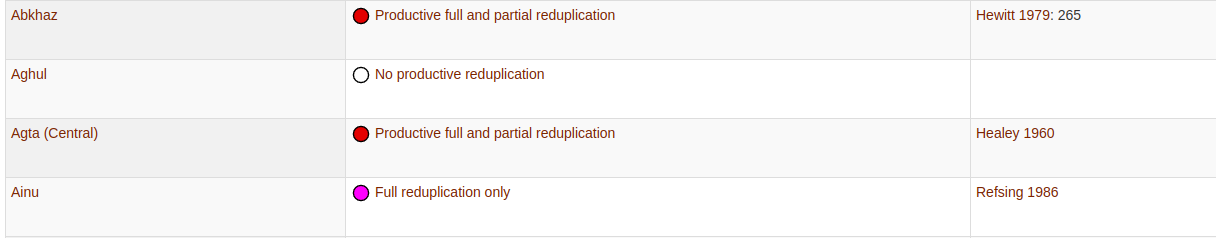
\includegraphics[width=13.5cm]{images/WALS.png}
\centering
\caption{A sample of WALS data on reduplication, available at https://wals.info/feature/27A, accessed 19 Nov 2019.}
\end{figure}

The World Atlas of Language Structures is "a large database of structural (phonological, grammatical, lexical) properties of languages gathered from descriptive materials (such as reference grammars) by a team of 55 authors." It contains information about twelve morphology features, such as "Reduplication," "Prefixing vs. Suffixing in Inflectional Morphology," and "Inflectional Synthesis of the Verb" \parencite{WALS}. Some of these may be measurable via analysis of the SIGMORPHON data as well, e.g., "Exponence of Tense-Aspect-Mood Inflection," "Prefixing vs. Suffixing in Inflectional Morphology," and "Case Syncretism," while others, such as "Reduplication" and "Locus of Marking in the Clause" would probably be harder to measure in such a way. For the features which can also be generated by looking at the SIGMORPHON data, the WALS data can at least be used as a gold standard to calibrate and assess the quality of generated metrics. WALS will not be useful in assessing overlap between sets of inflectional categories which are present or exhibit fusion in languages - its categorical tagging is simply not granular enough - but fortunately these will be relatively straightforward measures to generate from the SIGMORPHON 2018 data.

\subsection{Generated metrics}

Assessing set of inflectional categories and paradigm size based on the SIGMORPHON 2018 data will be very straightforward - I will simply need to list which UniMorph tags appear, and count the total number of UniMorph tag combinations seen, in each part of speech in each language.

To generate the other metrics, string alignment and transduction methods adopted from pre-neural morphology models will be necessary. Most clear is that to assess inflection shape, I will need to perform character alignment as in Figure 2.2 and count how many string changes take place before, after, or within the stem. 

To measure fusion between a pair of grammatical categories, average Levenshtein or LCS distance can be taken between forms that differ along both categories and compared to distance between forms that only differ along one category. For example, recall the Spanish verbs \textit{hablé} "I spoke", \textit{hablo} "I speak", \textit{habló} "he/she spoke". \textit{Hablé} differs from each of the other forms along one category - it has a different tense from \textit{hablo} and a different subject person than \textit{habló} - and its LCS distance from each is 2. \textit{Hablo} and \textit{habló} differ in both tense and subject person but also have a LCS distance of 2; the fact that forms that differ along both categories are no more dissimilar than forms that differ along one is an indicator of the fact that tense and subject agreement are fused in Spanish verbs. In contrast, consider the Finnish verbs \textit{puhuin} "I spoke", \textit{puhun} "I speak", and \textit{puhui} "he/she spoke" - \textit{puhuin} has an LCS distance of 1 from both other forms while they have an LCS distance of 2 from one another, indicating that in this case Finnish does not fuse tense and subject marking - past tense is constructed with a suffix \textit{-i} and first person subject with a subsequent suffix \textit{-n}.

Presence of long-distance phonological processes will be the most difficult to measure by analyzing the SIGMORPHON data. Fortunately, the presence of vowel and consonant harmony is typically quite binary and pervasive throughout a language's morphology, so rather than attempting to generate a measurement of it I may simply hand-annotate languages with a binary indication of whether or not they possess some long-distance process, and perhaps secondarily with a more specific indication of the type (e.g., frontness vowel harmony, sibilant harmony, etc.).
\chapter{Methods and Results}

\section{Assessing the impact of transfer learning}

There are no results available from SIGMORPHON that directly measure the impact of transfer learning while controlling for other model parameters. 

SIGMORPHON 2018 task 1 used a string transduction model as a baseline, and received a variety of submitted models which all used a neural component but many of which took advantage of ensembling with string transduction methods. It did not explicitly make transfer learning data available, though one team did use multilingual training data to build its model \parencite{Cotterell2018b}.

The goal of the SIGMORPHON 2019 task 1 was the same as SIGMORPHON 2018 - morphological inflection - but it was specifically a transfer learning task. For the source language, a high-resource data set was provided, and for the target language a low-resource data set; these data sets are identical in size and format to the 2018 high- and low-resource training sets, but they were resampled and so don't contain exactly the same data. SIGMORPHON 2019 provided four baseline models for task 1, all of which were purely neural and differed by attention mechanism, and all submissions were neural models \parencite{McCarthy2019}. 

Given the similarity of data and goals between SIGMORPHON 2018 and 2019, it may be surprising that, for 50 of the 100 training pairs, higher accuracy was achieved on the target language in low-resource settings by the best model of 2018 than by any submission in 2019. It might have been expected that with access to additional data, as well as information from the previous year about which models were successful, models in 2019 should have avoided declining performance. The reason for the performance declines may be that in 2018, the models that performed best in low-resource settings were actually quite different than those that scored well in high-resource settings. Models adapted to low-resource settings tended to avoid pure reliance on neural encoder-decoder models and used techniques such as using string transduction to learn edit sequences and string alignments, and biasing toward copying characters. With the task refocused on neural transfer learning in 2019, many of these techniques might have been dropped. It also may be the case that, since training sets were resampled from 2018 to 2019, the languages that saw worsened performance in 2019 simply had by random chance less useful training sets that year. The low-resource training sets in 2018 and 2019 were relatively small with at most 100 examples, making for greater likelihood of chance sampling effects (\cite{McCarthy2019}, \cite{Cotterell2018b}).

Despite the many confounding factors between the 2018 and 2019 best model performances, some suggestive results are yielded by comparing the best performance of any submission on each pair in 2019 to the best performance of any 2018 submission on the comparable task of modeling the pair's target language in a low-resource setting. Barring differences in modeling technique and data sampling, the two problems are essentially equivalent - using about 100 examples of a language to predict any other inflected form from that language - with the major difference being the transfer learning data, about 10,000 examples of a different language, that was made available in 2019. 

I looked at rudimentary typological, genealogical, and sampling metrics of the languages and training pairs to find correlations with model improvements between 2018 and 2019. The methods of generation of this data, and statistical analysis of it, are presented in this section; potential interpretations and implications are discussed in the next section.

\section{Genealogical distance}

SIGMORPHON 2019 stated that 20 of its 100 language pairs were distantly or unrelated, based on the language "family" designations in SIGMORPHON 2018. I used the Ethnologue language genealogy designations to generate a three-tiered distance designation: "Closely related" (in the same language family and subfamily), "Distantly related" (in different subfamilies of the same family), and "Unrelated" (in different families). By my designation, there are 62 closely related pairs, 31 distantly related pairs, and 7 unrelated pairs.

I conjecture that most distantly related pairs have dissimilar enough forms as to behave much more like unrelated languages with perhaps coincidental structural similarities than like closely related languages. However, my designations are not a fine-grained or necessarily consistent metric of actual similarity; some language families are much more internally diverse than others, and subfamily divisions were chosen somewhat arbitrarily. 

On average, more distantly related language pairs actually perform better and show more improvement between 2018 and 2019, perhaps suggesting that transfer learning between closely related languages confuses the model, although this result is not statistically significant.

\begin{figure}[ht]
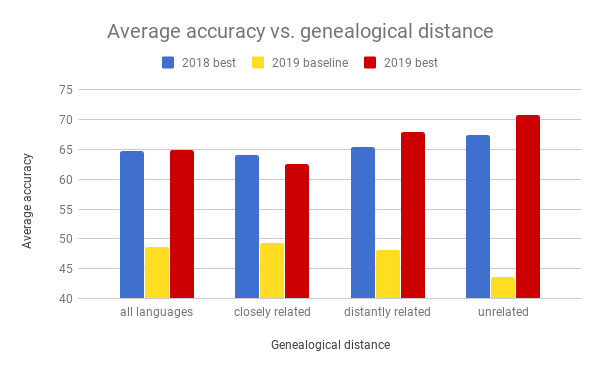
\includegraphics[width=12cm]{images/Average_accuracy_vs_genealogical_distance.png}
\centering
\end{figure}

I conducted all statistical tests on both the set of all language pairs and the set of all distantly related and unrelated language pairs, but no statistically significant results were achieved over the set of all language pairs; perhaps because genealogical relationship is too strong a confounding variable.

\section{Part of speech category overlap}

As discussed in the data section, the UniMorph annotations in the training data were scraped to discover the full set of morphological categories for which each part of speech could be inflected in each language. These category sets were used to generate a metric of structural similarity I call category overlap.

\subsection{Calculating overlap}

For each part speech in each of two languages, given the category sets $C_{POS, language\ A}$ and $C_{POS, language\ B}$, the overlap was calculated as

\[overlap(POS, language\ A, language\ B) = \frac{\abs*{C_{POS, language\ A}\ \cap\ C_{POS, language\ B}}}{\abs*{C_{POS, language\ A}\ \cup\ C_{POS, language\ B}}}\]

Take as an example the category overlap of nouns in German and Greek. The German category set for nouns is $C_{N,German} = \{ACC, DAT, GEN, NOM, PL, SG\}$ - German inflects nouns for singular and plural number and four grammatical cases. The Greek nominal category set is similar, except that it lacks a dative case and has a vocative case: $C_{N,Greek} = \{ACC, VOC, GEN, NOM, PL, SG\}$. The nominal category overlap is 

$overlap(N, German, Greek)$\\
$= \frac{\abs*{\{ACC, DAT, GEN, NOM, PL, SG\}\ \cap\ \{ACC, VOC, GEN, NOM, PL, SG\}}}{\abs*{\{ACC, DAT, GEN, NOM, PL, SG\}\ \cup\ \{ACC, VOC, GEN, NOM, PL, SG\}}}$\\
$= \frac{\abs*{\{ACC, GEN, NOM, PL, SG\}}}{\abs*{\{ACC, DAT, VOC, GEN, NOM, PL, SG\}}}$\\
$= \frac{5}{7} \approx .71$\\

It is not uncommon for one or both languages in a pair to lack any morphological categories for a particular part of speech; many languages do not have training data for all parts of speech. If only one language has an empty tagset for a part of speech, then by the above formula the category overlap is 0. If both languages have empty tagsets, the above formula would yield $\frac{0}{0}$, not a real number; in such a case the pair is excluded from analysis, which is why $n$ is less than the total number of language pairs in the findings below.

\subsection{Correlation with model performance}

Overall, verbal category overlap was much more predictive than nominal category overlap of performance changes between 2018 and 2019. In particular, the verbal category overlap of a transfer learning pair had a highly significant (p<.01) relationship with year over year accuracy improvement, with an additional .1 verbal category overlap score predicting a 3.7\% jump in absolute model accuracy between the two years. The relationship of nominal category overlap to model improvement did not rise to any significance threshold.

\begin{figure}[ht]
\includegraphics[width=12cm]{images/generated/significant/Accuracy_Improvement_vs_2018_vs_V_category_overlap_distantly_related_and_unrelated_language_pairs.png}
\centering
\caption{The relationship between a pair's verbal category overlap and the best team's performance in 2019 relative to 2018.}
\end{figure}

\begin{figure}[ht]
\includegraphics[width=12cm]{images/generated/insignificant/Accuracy_Improvement_vs_2018_vs_N_category_overlap_distantly_related_and_unrelated_language_pairs.png}
\centering
\caption{The relationship between a pair's nominal category overlap and the best team's performance in 2019 relative to 2018.}
\end{figure}

I used randomized permutation testing to approximate the significance level of the correlation.

\section{Part of speech distribution similarity}

The UniMorph tags identify four broad parts of speech cross-linguistically in the SIGMORPHON data: nouns, verbs, adjectives, and determiners. However, there is only one language among the 79 in the SIGMORPHON 2019 data that has all of these parts of speech represented; 64 languages have verb data, 55 have noun data, 40 have adjective data, and only 2 have determiner data. 

I use similarity between the relative distributions of parts of speech in source and target training sets as a metric of data set similarity. Part of speech distribution in the SIGMORPHON data is not necessarily an indication of actual linguistic typology; while some languages lack inflection on some parts of speech, there are also omissions in the SIGMORPHON data due to data sparsity \parencite{Cotterell2018b}.

\subsection{Calculating similarity}

My part of speech distribution similarity statistic is simply the statistical distance between the part of speech distributions of the two languages, calculated by summing the differences of the proportions of each part of speech between the two languages. That is, if $f_{POS, language}$ is the number of training forms for a given language and part of speech and $f_{language}$ is the total number of training forms for a language, the part of speech distribution similarity between language A and language B is

\[POSDS(language\ A, language\ B) = \sum\limits_{POS}\ \abs*{\frac{f_{POS, language\ A}}{f_{language\ A}} - \frac{f_{POS, language\ B}}{f_{language\ B}}}\]

where $POS = \{N, V, ADJ, DET\}$.

\subsection{Correlation with model performance}

\begin{figure}[ht]
\includegraphics[width=12cm]{images/generated/significant/Accuracy_Improvement_vs_2018_vs_POS_distribution_similarity_distantly_related_and_unrelated_language_pairs.png}
\centering
\caption{The relationship between a pair's part of speech distribution similarity and the best team's performance in 2019 relative to 2018.}
\end{figure}

Another significant (p<.05) negative relationship was discovered between part of speech distribution similarity and model improvement between 2018 and 2019. That is, the more that the data sets of source and target language for a given pair shared the same parts of speech, the worse a transfer learning model could be expected to perform relative to a 2018 non-transfer model. If models over transfer learning pairs with similar part of speech distributions actually performed worse overall, that would constitute evidence that a similar source and target domain somehow confused or worsened the model, and that transfer learning was thus counterproductive. However, there is no evidence of any relationship between data set similarity and \textit{overall} model performance:

\begin{figure}[ht]
\includegraphics[width=12cm]{images/generated/insignificant/Best_Transfer_Accuracy_vs_POS_distribution_similarity_distantly_related_and_unrelated_language_pairs.png}
\centering
\caption{The relationship between a pair's part of speech distribution similarity and the best team's performance in 2019.}
\end{figure}

Since transfer learning pairs with similar part of speech distributions could be modeled as well as other pairs in 2019, but showed less \textit{improvement} from transfer learning, the target languages of those pairs must have been more effectively modeled in 2018. Since transfer learning was not an available strategy in 2018, and only target language data was available, similarities between source and target data cannot directly explain this better performance in 2018. There must be some confounding factor accounted for the by selection of transfer learning pairs.
% \chapter{Conclusions and Discussion}

\section{Overall model accuracy disparities between languages}

One trend that plainly jumps out in the data from SIGMORPHON 2018 and 2019 is that some languages are persistently more difficult to model than others. 

In SIGMORPHON 2018 task 1 best achieved scores, the SIGMORPHON 2019 task 1 baseline models, and the SIGMORPHON 2019 best achieved scores, models of Old Irish always have the lowest accuracy rate, never higher than 10\%, typically followed in second or third place by Latin. 

On the other end of the spectrum, the Turkic languages included in the SIGMORPHON data (Azeri, Bashkir, Crimean Tatar, Kazakh, Khakas, Tatar, Turkish, Turkmen, Uzbek) have among the highest-accuracy models. In the SIGMORPHON 2018 task 1 with a low data setting, 6 of 9 featured Turkic languages achieved accuracies above 85\%, and the Turkic languages averaged 80\% accuracy while the overall mean accuracy was 62\%. In SIGMORPHON 2019 task 1, language pairs with a Turkic target language averaged 74\% baseline accuracy while the overall was 49\%, 81\% best accuracy where the average was 65\%. Curiously, the Turkic languages actually had slightly worse models on average in SIGMORPHON 2019 than 2018, while overall, the accuracy of best models for a given language held constant on average. (The reason that the average best score for Turkic languages was 81\% in 2019 compared to 80\% for 2018 is that higher-accuracy Turkic languages happened to be chosen more often as target languages for transfer pairs in 2019. Best model accuracy for individual Turkic languages decreased by an average of 3\% from 2018 to 2019.)

To some degree, these outcomes correspond with probably expected intuitions or general perceptions of the relevant languages. Turkic languages, for instance, are known for straightforward agglutinative morphology and almost entirely lacking declension classes and irregular forms; for a given grammatical meaning, there is typically a single suffix that is applied to all words \parencite{Johanson1998}. 

\subsection{CMU-03}

There are two language pairs that stand out as seeming outliers in the SIGMORPHON 2019 data, in different ways: Bengali $\rightarrow$ Greek and Swahili $\rightarrow$ Quechua. 

In 2018, the University of Zurich team achieved 32\% accuracy in modeling Greek with a low volume data, the best team on that problem. Greek $\rightarrow$ Bengali and Bengali $\rightarrow$ Greek pairs appeared in SIGMORPHON 2019. The Greek $\rightarrow$ Bengali pair scored fairly typically: the best 2019 model was slightly better than the 2019 baselines and slightly worse than the best 2018 low-resource Greek model. But the Bengali $\rightarrow$ Greek scored only 18\% accuracy from the best 2019 baseline model, yet the Carnegie Mellon team was able to achieve 75\% accuracy on that pair, by far the largest difference between a 2019 baseline and best team performance, and the second-highest absolute improvement between 2018 and 2019. The case of Swahili $\rightarrow$ Quechua is even more drastic: while the best 2019 baseline could only score 14\% accuracy, the same Carnegie Mellon model achieved 92\% accuracy, the single largest disparity between a 2019 baseline and best score.

That model, denoted \texttt{CMU-03} in \cite{McCarthy2019}, had the highest overall accuracy of all submitted models, and was the best performer on 61 of the 100 language pairs, but in particular performed comparatively well on pairs that had done poorly in 2018 or with the 2019 baseline models. \cite{McCarthy2019} et. al. also note that the success of \texttt{CMU-03} is correlated with linguistic similarity of the two languages, though these examples in particular do not provide evidence for that idea. Bengali $\rightarrow$ Greek is a quite distantly related pair, with the two languages belonging to different primary branches of the large and diverse Indo-European family, and Swahili $\rightarrow$ Quechua are completely unrelated. Bengali $\rightarrow$ Greek has fairly typical part of speech distribution overlap and nominal and verbal category overlap, while Swahili $\rightarrow$ Quechua scores substantially below average on all three similarity metrics.

\texttt{CMU-03} is unique in that it employs techniques to attend over morphological tags before ingesting the input lemma, and to bias toward character copying. The effect of these techniques is not clear, but provides an interesting area of future research. Unfortunately, there is no separately published paper or codebase for \texttt{CMU-03}.

\section{Overall outlook for transfer learning as a morphology learning strategy}

\cite{McCarthy2019} states that "gains from cross-lingual training were generally modest, with gains positively correlating with the linguistic similarity of the two languages." The claim that using transferred knowledge boosts model performance, if slightly, seems to come from individual reports from teams about their models. Unfortunately, code or full results for the individual 2019 SIGMORPHON task 1 submissions were not published, so to verify the claim, a comparison of models that differ only in their use of transfer knowledge must be conducted. According to comparison of 2018 and 2019 best models, however, average model performance with or without access to transfer learning was essentially the same, while best model performance varied widely between different pairs.

Given the similarity of data and goals between SIGMORPHON 2018 and 2019, it may be surprising that, for 50 of the 100 training pairs, higher accuracy was achieved on the target language in low-resource settings by the best model of 2018 than by any submission in 2019. It might have been expected that with access to additional data, as well as information from the previous year about which models were successful, models in 2019 should have avoided declining performance. The reason for the performance declines may be that in 2018, the models that performed best in low-resource settings were actually quite different than those that scored well in high-resource settings. Models adapted to low-resource settings tended to avoid pure reliance on neural encoder-decoder models and used techniques such as using string transduction to learn edit sequences and string alignments, and biasing toward copying characters. With the task refocused on neural transfer learning in 2019, many of these techniques might have been dropped. Since all team performances on SIGMORPHON 2019 task 1 were not published, it is not possible to assess the impact of particular model parameters on performance with different types of languages. 

It also may be the case that, since training sets were resampled from 2018 to 2019, the languages that saw worsened performance in 2019 simply had by random chance less useful training sets that year. The low-resource training sets in 2018 and 2019 were relatively small with at most 100 examples, making for greater likelihood of chance sampling effects.

As shown in section 5, from comparison of 2018 and 2019 data, it is far from clear that genealogical relationship between languages leads to effective transfer learning, while verbal category overlap does seem to be significantly predictive of better transfer learning. The statistically significant negative relationship between part of speech distribution similarity and model performance, as well as the suggestive but not statistically significant negative relationship between genealogical closeness and model performance, suggests that transfer knowledge may actually be capable of \textit{confusing} a model. 

% \section{The relationship between category overlap and transfer learning success}


% \section{The relationship between POS distribution similarity and transfer learning success}

\section{Potential language pair sampling confounds}

\subsection{Language pair sampling}

Language pairs for SIGMORPHON 2019 were not selected at random from an even distribution. Many languages appear only as target languages because they lack high-volume data, and some of the languages from the SIGMORPHON 2018 data appear in as many as 5 pairs while others were not included. Some groups of languages, such as Germanic and Turkic groups, appear to have been near-exhaustively paired between a subset of source and a subset of target languages, while the number of fully unrelated pairs is just 7. Genealogical relationship between a language pair appears to be a substantial confound - many results appear statistically significant among non-closely related languages, while no statistically significant inferences could be drawn about the entire pool of language pairs.

\subsection{Turkic languages}

Particular language families also differ from one another, both in internal diversity and in typological trends. In particular, the Turkic family stood out as an outlier in the SIGMORPHON 2019 data. As noted in 6.1, Turkic languages share a set of morphological characteristics that make them relatively easy to model accurately, as evidenced by the higher-than-average accuracy of models over the Turkic languages. The Turkic language family may also be an instance of a family with less internal diversity than, say, the Indo-European family. 

\begin{figure}[ht]
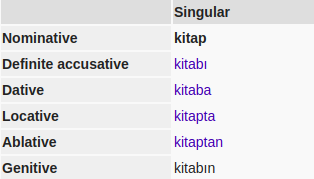
\includegraphics[width=8cm]{images/Turkish_kitap.png}
\centering
\caption{Nominal declension in Turkish, an Oghuz Turkic language (Wiktionary).}
\end{figure}

\begin{figure}[ht]
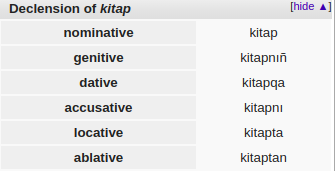
\includegraphics[width=8cm]{images/Crimean_Tatar_kitap.png}
\centering
\caption{Nominal declension in Crimean Tatar, a Kipchak Turkic language (Wiktionary).}
\end{figure}

\begin{figure}[p]
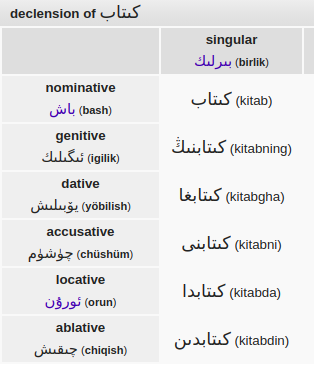
\includegraphics[width=8cm]{images/Uyghur_kitap.png}
\centering
\caption{Nominal declension in Uyghur, a Karluk Turkic language (Wiktionary).}
\end{figure}

For instance, the above declension tables for the word \textit{kitap} "book" show that three languages from different primary branches of the Turkic family all share the same set of noun cases, with cognate suffixes.

Contrast this with inflection of the respective words for "book" in Swedish and Czech, two Indo-European languages of different subfamilies.

\begin{figure}[p]
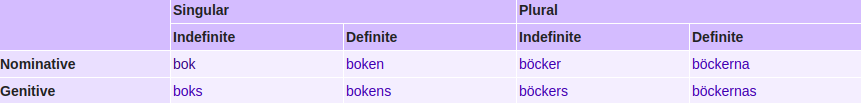
\includegraphics[width=13cm]{images/Swedish_bok.png}
\centering
\caption{Nominal declension in Swedish, a Germanic Indo-European language (Wiktionary).}
\end{figure}

\begin{figure}[p]
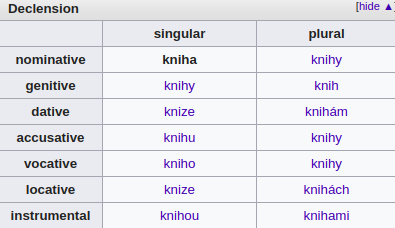
\includegraphics[width=8cm]{images/Czech_kniha.png}
\centering
\caption{Nominal declension in Czech, a Slavic Indo-European language (Wiktionary).}
\end{figure}

\newpage

Given that removing closely related languages from consideration was necessary to generate any statistically significant results, if Turkic languages are designated as "Distantly related" while being quite similar, this might obscure otherwise significant results. And indeed, that seems to have occurred in at least one place: a statistically significant (p<.05) relationship emerges between genealogical distance and model performance. If all language pairs with Turkic target languages are removed from the data set, and genealogical distance is mapped onto a continuous space from 0 (different language family) to 1 (different subfamilies of the same language family) to 2 (same family and subfamily), the previously non-significant negative relationship between genealogical closeness and model performance appears to be statistically confirmed. This result implies that transferred knowledge about a genealogically related source language actually somehow hinders or confuses a model of a target language, contrary to the conclusions of \cite{McCarthy2019}.

\begin{figure}[ht]
\includegraphics[width=12cm]{images/generated/significant/Accuracy_Improvement_vs_2018_vs_Genealogical_distance_non-Turkic_languages.png}
\centering
\caption{Language pair genealogical similarity has a significant negative relationship with model performance once Turkic languages are removed from the data set.}
\end{figure}

This study does not currently possess systematic evidence that the Turkic language family is less diverse than other included language families. Finding a way to include measures of lexical similarity or otherwise measure language relatedness in a more refined way would allow for much more effective and convincing amelioration of the confounding effect of linguistic genealogical relationships.
%\pdfbookmark[0]{Appendix}{Appendix}
\chapter{Appendix: compiled linguistic typology data}
\label{sec:Appendix}
\vspace*{-10mm}



%\cleardoublepage

% --------------------------
% Back matter
% --------------------------
{%
\setstretch{1.1}
\renewcommand{\bibfont}{\normalfont\small}
\setlength{\biblabelsep}{0pt}
\setlength{\bibitemsep}{0.5\baselineskip plus 0.5\baselineskip}
\printbibliography[nottype=online]
\printbibliography[heading=subbibliography,title={Webseiten},type=online,prefixnumbers={@}]
}
 \cleardoublepage

%\listoffigures


% % \listoftables
% \cleardoublepage

% % \input{content/colophon}
% \cleardoublepage

% \input{content/declaration}

% \newpage
% \mbox{}

% **************************************************
% End of Document CONTENT
% **************************************************
\end{document}
